\documentclass[11pt]{article}

\usepackage[utf8]{inputenc}
\usepackage[T1]{fontenc}
\usepackage{lmodern}
\usepackage[margin=1in]{geometry}
\usepackage{amsmath,amssymb,mathtools,bm}
\usepackage{booktabs,array,tabularx}
\usepackage{graphicx}
\usepackage{microtype}
\usepackage{xcolor}
\usepackage{enumitem}
\usepackage{hyperref}
\usepackage{cleveref}
\usepackage{tikz}
\usetikzlibrary{arrows.meta,positioning,fit,calc}

\hypersetup{
  colorlinks=true,
  linkcolor=blue!50!black,
  citecolor=blue!50!black,
  urlcolor=blue!50!black
}

\newcommand{\E}{\mathbb{E}}
\newcommand{\Var}{\operatorname{Var}}
\newcommand{\diag}{\operatorname{diag}}
\newcommand{\R}{\mathbb{R}}
\newcommand{\pos}[1]{\left[#1\right]_+}
\newcommand{\given}{\,\middle|\,}

\title{\textbf{Denoise First, Differentiate Second}\\
Stable Latent-Dynamics Recovery for Neural Imaging}
\author{
Raul Valle \and Jos\'e C. Principe\\
Department of Electrical and Computer Engineering\\
University of Florida
}
\date{Working draft --- July 27, 2026}

\begin{document}
\maketitle

\begin{abstract}
Temporal differencing is attractive in neural imaging because persistent anatomy
and illumination cancel while rapid fluorescence changes remain. In NeuRev,
two-observation InfoMax and Cauchy--Schwarz Parzen separation empirically
recovered directions nearly identical to adjacent-frame subtraction. This is a
useful result, but it also clarifies the limitation: pairwise source separation
has mostly learned a temporal derivative. Differencing a noisy movie amplifies
independent frame noise, suppresses slow calcium dynamics, reacts to motion
edges, and discards absolute fluorescence. We therefore propose a different
scientific order. First estimate a stable latent fluorescence trajectory from an
explicit observation model; then derive ordinary differences, model-aware
dynamic drives, and prediction residuals as separate downstream features. A
linear Gaussian autoregressive state-space model provides the first falsifiable
reference, with a causal Kalman filter and an offline Rauch--Tung--Striebel
smoother. The key feature is
\(u_t=s_t-\gamma s_{t-1}\), which generalizes the subtraction direction
\([-1,1]\) to the dynamics-aware direction \([-\gamma,1]\). The framework
separates denoising from event extraction, makes stability and uncertainty
explicit, and admits stronger extensions such as robust state-space models,
local dynamic factors, sparse calcium-drive inference, penalized matrix
decomposition, and self-supervised video denoising. We present the canonical
argument, the proposed NeuRev implementation, and a falsification-oriented
evaluation program.
\end{abstract}

\section{The problem in one picture}

The practical objective is not to manufacture the smoothest possible movie. It
is to estimate the fluorescence dynamics that are supported by the observation
while suppressing stochastic measurement noise and exposing model failure.

\begin{figure}[h]
\centering
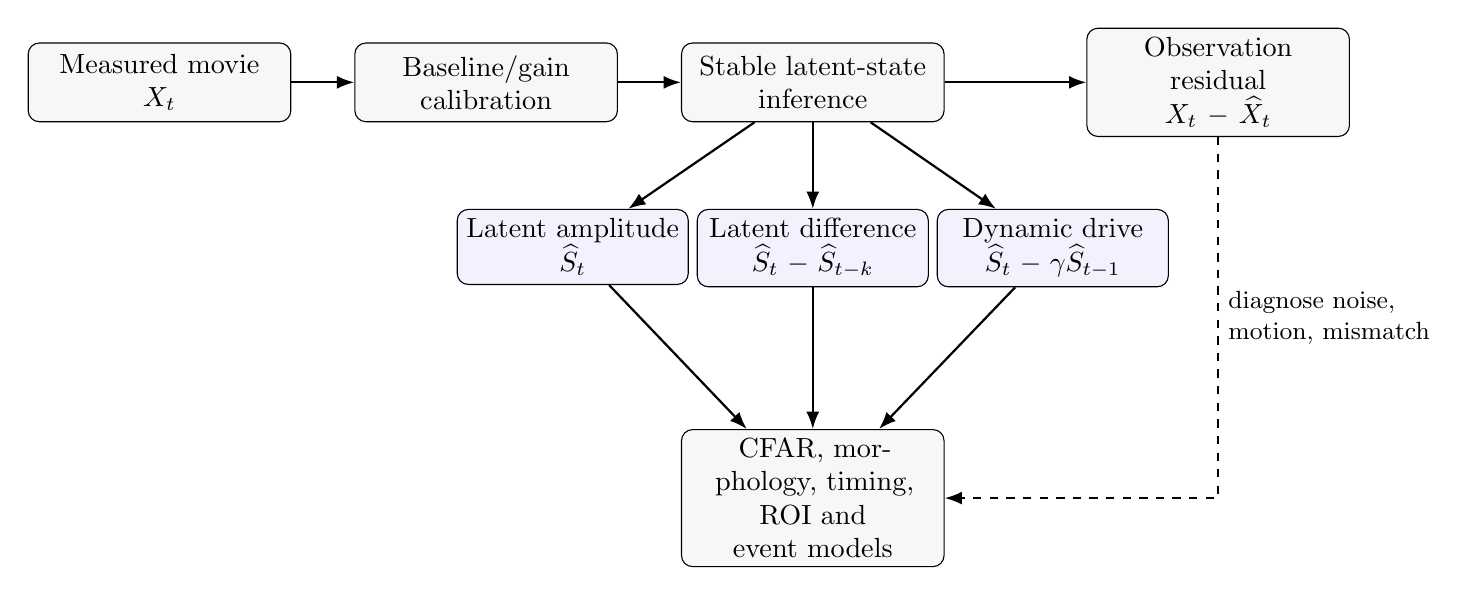
\begin{tikzpicture}[
  node distance=7mm and 8mm,
  box/.style={draw, rounded corners, align=center, minimum height=10mm,
              text width=31mm, fill=black!3},
  feature/.style={draw, rounded corners, align=center, minimum height=9mm,
                  text width=27mm, fill=blue!5},
  arrow/.style={-{Latex[length=2.2mm]}, thick}
]
\node[box] (raw) {Measured movie\\$X_t$};
\node[box, right=of raw] (cal) {Baseline/gain\\calibration};
\node[box, right=of cal] (state) {Stable latent-state\\inference};
\node[feature, below left=11mm and -1mm of state] (amp) {Latent amplitude\\$\widehat S_t$};
\node[feature, below=11mm of state] (diff) {Latent difference\\$\widehat S_t-\widehat S_{t-k}$};
\node[feature, below right=11mm and -1mm of state] (drive) {Dynamic drive\\$\widehat S_t-\gamma\widehat S_{t-1}$};
\node[box, right=18mm of state] (resid) {Observation residual\\$X_t-\widehat X_t$};
\node[box, below=18mm of diff] (down) {CFAR, morphology, timing,\\ROI and event models};

\draw[arrow] (raw) -- (cal);
\draw[arrow] (cal) -- (state);
\draw[arrow] (state) -- (amp);
\draw[arrow] (state) -- (diff);
\draw[arrow] (state) -- (drive);
\draw[arrow] (state) -- (resid);
\draw[arrow] (amp) -- (down);
\draw[arrow] (diff) -- (down);
\draw[arrow] (drive) -- (down);
\draw[arrow, dashed] (resid) |- node[pos=.25, right, align=left, font=\small]
  {diagnose noise,\\motion, mismatch} (down.east);
\end{tikzpicture}
\caption{The proposed order. Denoising estimates a latent trajectory; feature
extraction is a separate downstream operation. The residual remains visible as
a diagnostic rather than being silently discarded.}
\label{fig:pipeline}
\end{figure}

This ordering is the central proposal. It differs from a direct
entropy-maximizing inverse, which maps the observation to an output and then
rewards a desired output statistic. Here, a candidate latent signal must explain
the measured movie through an explicit forward model.

\section{What NeuRev has already taught us}

NeuRev's recent pairwise experiment starts with two observations at each spatial
sample:
\begin{equation}
\bm x_t(p)
=
\begin{bmatrix}
I_{t-1}(p)\\
I_t(p)
\end{bmatrix}.
\end{equation}
If persistent anatomy and illumination contribute almost equally to both
frames, their direction is approximately
\([1,1]^\top\). The orthogonal background-null direction is
\([-1,1]\), giving
\begin{equation}
[-1,1]\bm x_t(p)=I_t(p)-I_{t-1}(p).
\end{equation}

The fitted InfoMax and Cauchy--Schwarz Parzen directions in the first Spon Ca
Burst run were nearly collinear with this subtraction direction. This should not
be described as a failure. It is a precise empirical finding:

\begin{quote}
With only adjacent observations and a strongly persistent common component,
pairwise separation naturally becomes a temporal derivative.
\end{quote}

The next experiment then treated the continuous derivative/ICA values as
auxiliary channels for Raw Direct. Fixed additive fusion, a bounded learned
scalar fusion, and soft image gates did not improve the frozen Raw Direct
detector under held-out evaluation. More aggressive gates removed known
activity. This establishes a second result:

\begin{quote}
Change evidence is informative, but change alone is not a replacement for
absolute fluorescence and anatomical context.
\end{quote}

The remaining question is whether the derivative becomes more useful after the
underlying trajectory is denoised.

\section{Why raw differencing is both useful and dangerous}

Consider a simple observation
\begin{equation}
x_t=s_t+\epsilon_t,
\end{equation}
where \(s_t\) is the latent fluorescence and \(\epsilon_t\) is independent,
zero-mean frame noise with variance \(\sigma^2\). The raw first difference is
\begin{equation}
\Delta x_t
=
x_t-x_{t-1}
=
\Delta s_t+\epsilon_t-\epsilon_{t-1}.
\end{equation}
If the noise is independent across frames,
\begin{equation}
\Var(\epsilon_t-\epsilon_{t-1})=2\sigma^2.
\label{eq:noise-doubling}
\end{equation}
Thus subtraction cancels persistent structure but doubles the variance of white
frame noise.

This explains the visual character of derivative movies: static anatomy fades,
but high-frequency grain and edge flicker become prominent. The problem is
worse when the movie contains geometric motion. A small translation turns every
strong spatial edge into a paired positive/negative temporal edge, even when no
neuron fires.

Differencing also attenuates slow activity. A calcium transient that rises over
many frames may have substantial absolute amplitude but a modest frame-to-frame
change. A hard derivative gate can therefore erase the plateau and much of the
rise. NeuRev's completed activity-gating experiments exhibited exactly this
failure mode.

The correct conclusion is not that differencing is useless. It is that
differencing is a \emph{feature operator}, and its input matters.

\section{What should be denoised?}

A useful conceptual decomposition is
\begin{equation}
X_t(p)
=
G_t(p)+S_t(p)+N_t(p)+A_t(p),
\label{eq:decomposition}
\end{equation}
where:
\begin{itemize}[leftmargin=*]
\item \(G_t\) is baseline, illumination, persistent anatomy, and slow drift;
\item \(S_t\) is the latent fluorescence signal of interest;
\item \(N_t\) is stochastic measurement noise;
\item \(A_t\) is unmodeled artifact, including motion and saturation.
\end{itemize}

No temporal denoiser can guarantee a perfect separation of these terms from one
movie. The model must declare what it regards as persistent state, process
variation, observation noise, and artifact. The first NeuRev implementation
should therefore begin with a conservative baseline/gain calibration and model
the signed residual
\begin{equation}
r_t(p)=s_t(p)+\epsilon_t(p).
\label{eq:residual-model}
\end{equation}
The residual should remain signed during inference. Positive clipping is a
downstream visualization or detection choice:
\begin{equation}
a_t(p)=\pos{\widehat s_t(p)}.
\end{equation}

The method should output four objects, not one ambiguous ``cleaned'' movie.

\subsection{Latent state}

\begin{equation}
\widehat s_t
\end{equation}
is the denoised fluorescence trajectory. It should preserve slow evolution,
amplitude, duration, and spatial localization.

\subsection{State difference}

\begin{equation}
d_t^{(k)}
=
\widehat s_t-\widehat s_{t-k}
\end{equation}
is a lag-\(k\) change feature. In the Spon movie, \(k=1\) corresponds to
\(20\) ms and \(k=4\) to \(80\) ms.

\subsection{Dynamic drive}

If the latent state obeys a fitted autoregression, then
\begin{equation}
\widehat u_t
=
\widehat s_t-\gamma\widehat s_{t-1}
\label{eq:drive}
\end{equation}
is the part not explained by expected persistence. This is the
dynamics-aware generalization of subtraction.

\subsection{Observation residual}

\begin{equation}
e_t=r_t-\widehat s_t
\end{equation}
is what the smoother does not explain. It is not automatically noise.
Spatially or temporally structured residuals can indicate motion, saturation,
model mismatch, or neural activity that the model has erased.

\section{The first falsifiable model}

The recommended reference is a stable scalar AR(1) state-space model:
\begin{align}
s_t &= \gamma s_{t-1}+u_t,
&
u_t &\sim\mathcal N(0,q), \label{eq:state}\\
r_t &= s_t+\epsilon_t,
&
\epsilon_t &\sim\mathcal N(0,r), \label{eq:obs}
\end{align}
with \(0\leq\gamma<1\).

Here the first noise term should be read as the state drive \(u_t\); the
implementation brief requires the unambiguous name `dynamic_drive` for derived
outputs. This is not proposed because all calcium dynamics are truly Gaussian
or first-order. It is proposed because:

\begin{enumerate}[leftmargin=*]
\item the assumptions are explicit;
\item inference is exact under those assumptions;
\item stability is easy to enforce;
\item uncertainty is available;
\item causal and offline outputs can be compared;
\item and failure can be diagnosed rather than hidden inside a large network.
\end{enumerate}

\subsection{Kalman filtering}

Let
\(\widehat s_{t|t-1}\) and \(P_{t|t-1}\) denote the predicted mean and
variance before seeing \(r_t\). The scalar prediction is
\begin{align}
\widehat s_{t|t-1}
&=
\gamma\widehat s_{t-1|t-1},\\
P_{t|t-1}
&=
\gamma^2P_{t-1|t-1}+q.
\end{align}
The measurement prediction error, conventionally called the Kalman
\emph{innovation}, is
\begin{equation}
\nu_t
=
r_t-\widehat s_{t|t-1},
\end{equation}
with variance
\begin{equation}
F_t=P_{t|t-1}+r.
\end{equation}
The gain and posterior update are
\begin{align}
K_t&=\frac{P_{t|t-1}}{F_t},\\
\widehat s_{t|t}
&=
\widehat s_{t|t-1}+K_t\nu_t,\\
P_{t|t}
&=
(1-K_t)^2P_{t|t-1}+K_t^2r.
\label{eq:joseph}
\end{align}
Equation~\eqref{eq:joseph} is the scalar Joseph form, which makes the
nonnegativity of the covariance update explicit.

The filter computes a causal estimate using observations through time \(t\).
It is therefore the relevant reference for any eventual real-time NeuRev
pipeline.

\subsection{Rauch--Tung--Striebel smoothing}

For an offline recording, future frames can improve the estimate of an earlier
state. Starting from the filtered sequence, the backward smoothing gain is
\begin{equation}
J_t
=
\frac{P_{t|t}\gamma}{P_{t+1|t}}.
\end{equation}
The smoothed mean and variance satisfy
\begin{align}
\widehat s_{t|T}
&=
\widehat s_{t|t}
+
J_t
\left(
\widehat s_{t+1|T}-\widehat s_{t+1|t}
\right),\\
P_{t|T}
&=
P_{t|t}
+
J_t^2
\left(
P_{t+1|T}-P_{t+1|t}
\right).
\end{align}

The smoother is often a better scientific denoiser, but it is noncausal. It may
move evidence backward in time. NeuRev must therefore report filter and smoother
onset timing separately and must never expose the smoother as a real-time lane.

\subsection{Stable parameterization}

A fitted autoregression should not be stabilized only by clipping after an
optimizer step. A strict parameterization is
\begin{equation}
\gamma
=
(1-\varepsilon)\operatorname{sigmoid}(\theta),
\end{equation}
or, for a nonnegative decay process,
\begin{equation}
\gamma
=
\exp\left(-\frac{\Delta t}{\tau}\right),
\qquad
\tau_{\min}\leq\tau\leq\tau_{\max}.
\end{equation}
Process and observation variances should likewise be bounded away from zero.
Fits that repeatedly occupy several bounds should be reported as degenerate
rather than quietly accepted.

\section{Differencing after state estimation}

The state equation yields
\begin{equation}
u_t=s_t-\gamma s_{t-1}.
\end{equation}
Ordinary differencing gives
\begin{align}
\Delta s_t
&=s_t-s_{t-1}\\
&=u_t+(\gamma-1)s_{t-1}\\
&=u_t-(1-\gamma)s_{t-1}.
\label{eq:diff-drive}
\end{align}
Equation~\eqref{eq:diff-drive} is the key conceptual bridge.

If \(\gamma\approx1\), the dynamic drive and ordinary difference are similar.
This is the persistent-background regime in which pairwise ICA naturally
discovers \([-1,1]\). If \(\gamma<1\), ordinary differencing mixes the new drive
with the expected decay of the previous state. The model-aware feature
\([-\gamma,1]\) attempts to remove that predictable decay.

\begin{figure}[h]
\centering
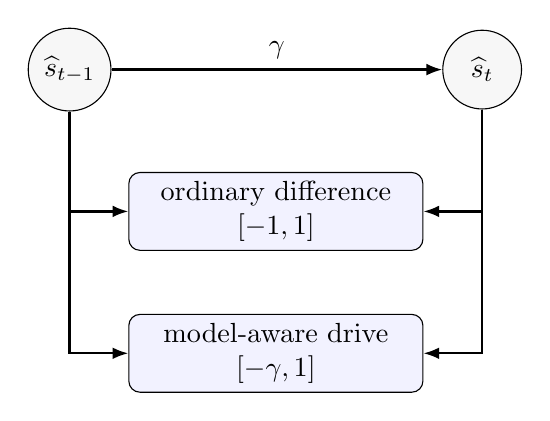
\begin{tikzpicture}[
  node distance=10mm and 12mm,
  state/.style={draw, circle, minimum size=10mm, fill=black!3},
  op/.style={draw, rounded corners, align=center, minimum height=9mm,
             text width=35mm, fill=blue!5},
  arrow/.style={-{Latex[length=2mm]}, thick}
]
\node[state] (prev) {$\widehat s_{t-1}$};
\node[state, right=42mm of prev] (curr) {$\widehat s_t$};
\node[op, below=13mm of $(prev)!0.5!(curr)$] (ordinary)
  {ordinary difference\\$[-1,1]$};
\node[op, below=8mm of ordinary] (model)
  {model-aware drive\\$[-\gamma,1]$};

\draw[arrow] (prev) -- node[above] {$\gamma$} (curr);
\draw[arrow] (prev) |- (ordinary.west);
\draw[arrow] (curr) |- (ordinary.east);
\draw[arrow] (prev) |- (model.west);
\draw[arrow] (curr) |- (model.east);
\end{tikzpicture}
\caption{Ordinary subtraction assumes perfect persistence. A fitted state model
replaces that assumption with a stable persistence coefficient \(\gamma\).}
\label{fig:gamma-difference}
\end{figure}

This does not guarantee that \(\widehat u_t\) is a neural firing event. It is a
model-relative temporal feature. Motion, unmodeled kinetics, and parameter
error can also appear as dynamic drive.

\section{Why the existing NeuRev ``Kalman'' result is not this test}

NeuRev currently contains a function named
\texttt{kalman\_positive\_residual\_stack}. It initializes a baseline from a
quiet median, computes the positive part of each frame-minus-baseline
difference, and updates the baseline with asymmetric fixed gains. Positive
changes are learned slowly; negative changes are learned more quickly.

That method can be useful, but it is best described as a
\emph{legacy asymmetric adaptive baseline}:

\begin{itemize}[leftmargin=*]
\item it does not maintain a model-based state covariance;
\item it does not estimate process and observation noise;
\item it does not compute a predictive likelihood;
\item it does not produce a fitted latent dynamical state;
\item and it does not provide an RTS smoother or posterior uncertainty.
\end{itemize}

A later NeuRev diagnostic passed this positive residual through spatial and
temporal Gaussian smoothing, quiet-period MAD whitening, and a learned local
contrast detector. That compound lane performed poorly. The valid conclusion
is that the \emph{compound preprocessing-plus-detector} was harmful. It does not
establish that a signed, likelihood-based state estimator is harmful.

The new experiment must retain this historical lane as a baseline and avoid
rewriting completed evidence. New reports should call it
\texttt{legacy\_asymmetric\_ema} while preserving the existing API and artifact
provenance.

\section{A hierarchy of candidate solutions}

No single denoising method dominates under every signal, noise, motion, and
latency regime. The methods answer different questions.

\begin{table}[h]
\centering
\small
\begin{tabularx}{\textwidth}{>{\raggedright\arraybackslash}p{0.20\textwidth}
                            >{\raggedright\arraybackslash}X
                            >{\raggedright\arraybackslash}X}
\toprule
Method & Main advantage & Main limitation \\
\midrule
Stable AR filter/smoother
& Explicit dynamics, exact linear-Gaussian inference, uncertainty, causal and
  offline forms
& Shared first-order Gaussian dynamics can oversmooth abrupt or heterogeneous
  neural activity \\
Robust state-space model
& Downweights impulsive/heavy-tailed observation errors
& Non-Gaussian inference and parameter fitting are more complex \\
Sparse nonnegative dynamics
& Matches calcium-like positive drives; OASIS provides efficient trace
  deconvolution~\cite{friedrich2017oasis}
& Requires a meaningful trace or spatial component and a justified kinetic
  model \\
Local dynamic factor model
& Uses spatial redundancy while modeling temporal dynamics in a compact state
& Rank, tiling, identifiability, and optimization require careful controls \\
Penalized matrix decomposition
& Scalable localized low-rank denoising for imaging data
  \cite{buchanan2018pmd}
& Primarily a denoiser; temporal event semantics require a second model \\
Self-supervised video denoising
& Can learn signal structure without clean targets
  \cite{batson2019noise2self,lecoq2021deepinterpolation}
& Depends on noise-independence and data-distribution assumptions; can suppress
  or invent structure under mismatch \\
CNMF
& Jointly models spatial footprints, temporal activity, background, and
  deconvolution~\cite{pnevmatikakis2016cnmf}
& More appropriate for cell/trace extraction than for a generic first
  denoised-movie reference \\
InfoMax / kernel dependence
& Useful higher-order criterion for source or innovation structure
& Does not by itself define the observation model, ensure stable inversion, or
  distinguish signal from generated high-entropy output \\
\bottomrule
\end{tabularx}
\caption{Candidate methods should be compared by the problem they solve rather
than placed under one generic ``denoising'' label.}
\label{tab:methods}
\end{table}

\subsection{The closest integrated extension}

After the scalar/tilewise reference is trustworthy, the strongest integrated
NeuRev extension is a local dynamic factor model:
\begin{align}
\bm x_t &= C\bm z_t+\bm\epsilon_t,\\
\bm z_t &= A\bm z_{t-1}+\bm u_t.
\end{align}
Here \(\bm x_t\) is an image patch, \(C\) is a spatial loading matrix, and
\(\bm z_t\) is a low-dimensional temporal state. Stable \(A\) models the
dynamics; \(C\) uses neighboring pixels to distinguish coherent signal from
pixelwise noise.

This is closer to an ``all-in-one'' denoiser because it uses both spatial and
temporal structure. It is still not universal. A patch model can mix multiple
neurons, absorb motion, choose an incorrect rank, or generate prior-dominated
content. It should therefore be introduced only after the reference model and
evaluation machinery are reliable.

\section{The proposed NeuRev experiment}

The implementation should proceed in stages.

\subsection{Stage 0: preserve anchors}

Reproduce Raw Direct exactly. Preserve completed frame-difference, pairwise,
learnable-contrast, and causal-proposal outputs. Maintain the rule that sparse
positive labels do not define exhaustive negatives.

\subsection{Stage 1: estimate observation noise}

Use only the declared quiet interval to estimate a per-pixel center and robust
scale. A conservative high-frequency estimate is
\begin{equation}
\widehat r(p)
\approx
\frac{1}{2}
\Var_{\rm robust}
\left(
r_t(p)-r_{t-1}(p)
\right).
\end{equation}
Slow quiet dynamics can make this an overestimate; the diagnostic must say so.
Normalize pixels by the quiet scale before fitting shared dynamics.

\subsection{Stage 2: fit a bounded AR(1) reference}

Fit \(\gamma\) and a bounded process-to-observation variance ratio on a
deterministic spatial sample using blocked predictive likelihood. Labels must
not choose the denoiser. A bounded grid should precede EM so the first
implementation has an auditable reference and cannot disappear into an
unstable optimizer.

\subsection{Stage 3: apply filter and smoother}

Apply the selected model in bounded image tiles. Save the causal filter mean,
offline smoother mean, compact covariance sequence, model parameters, and
diagnostics. Dense residuals and duplicate feature stacks should not be written
unless preregistered.

\subsection{Stage 4: derive a feature bank}

Derive in chunks:
\begin{align}
a_t &= \pos{\widehat s_t},\\
d_t^{(1)} &= \widehat s_t-\widehat s_{t-1},\\
d_t^{(4)} &= \widehat s_t-\widehat s_{t-4},\\
u_t &= \widehat s_t-\gamma\widehat s_{t-1},\\
z_{\nu,t} &= \nu_t/\sqrt{F_t}.
\end{align}
Keep signed and positive views distinct. A binary mask is a thresholded decision
artifact, not the preferred scientific representation.

\subsection{Stage 5: evaluate denoising before detection}

The first report should establish whether the latent trajectory is valid.
Only then should existing temporal pooling, quiet-only threshold calibration,
nonmaximum suppression, and known-label matching be applied to each feature.

Do not begin with a learned fusion. First ask which individual features carry
useful evidence. A later fusion may start exactly at Raw Direct with all
auxiliary weights at zero.

\section{Stability is a multi-part requirement}

\subsection{Dynamical stability}

For AR(1), require \(|\gamma|\leq1-\varepsilon\). For AR(2) or a matrix state,
require a strict Schur margin or an equivalent Lyapunov/contraction
certificate. A stable state model should remain bounded under a bounded
constant input.

\subsection{Numerical stability}

Use finite variance floors, float64 covariance recursions, a
positive-semidefinite covariance update, log-domain likelihood accumulation,
and explicit NaN/Inf checks. Save gain and variance extrema. A run that
completes with a collapsed covariance is not successful.

\subsection{Inverse and denoising stability}

Small changes in the movie or calibration should not create large changes in
the latent trajectory. Evaluate deterministic noise realizations, modest gain
drift, heteroscedastic noise, and model mismatch. Report the distribution of
output changes, not only one selected run.

\subsection{Statistical stability}

Fit parameters on blocked temporal subsets and deterministic spatial samples.
Report parameter and feature variation across blocks and seeds. The current
dataset contains only four labeled burst windows; conclusions should emphasize
effect size and fold consistency rather than asymptotic significance.

\subsection{Scientific stability}

A method is scientifically unstable if small hyperparameter changes cause
different neurons, onset times, or candidate rankings even when its numerical
loss is smooth. NeuRev should report candidate overlap and known-event
preservation across nearby model parameters.

\section{Identifiability and uncertainty}

A state-space model does not create information. It combines measurements with
a prior over dynamics. Where the observation is weak, the posterior estimate is
more prior-dependent.

This distinction is especially important for denoising. A plausible output is
not necessarily a uniquely recovered signal. Posterior variance, filter-smoother
disagreement, residual structure, and sensitivity to the prior should remain
visible.

If two latent trajectories produce the same observation under the admissible
forward model, no deterministic postprocessing can determine which one
occurred. A nonlinear network can generate a completion, but that completion is
conditioned on its learned prior. NeuRev should use the terms
\emph{prior-conditioned estimate} or \emph{completion}, not
\emph{recovered information}, in such regimes.

\section{Falsification-oriented evaluation}

A denoiser should be tested on cases designed to make it fail.

\subsection{Synthetic and semi-synthetic data}

Use noise-free ground truth for:
\begin{itemize}[leftmargin=*]
\item constant signals with white noise;
\item known AR(1) and AR(2) dynamics;
\item positive events with known onset, rise, plateau, and decay;
\item slow ramps;
\item closely spaced events;
\item pure noise;
\item impulsive and heteroscedastic noise;
\item gain and offset drift;
\item synthetic translation edges;
\item and mismatched decay constants.
\end{itemize}

Inject soma-like spatial patterns into real quiet Spon frames so the noise and
anatomical background remain realistic.

Required metrics include latent NMSE, amplitude bias, onset error, duration
bias, residual autocorrelation, uncertainty coverage, quiet false-event count,
parameter error, and event-to-quiet separation of both ordinary difference and
dynamic drive.

\subsection{Real-data signal preservation}

Before candidate detection, compare raw, latent, residual, difference, and
dynamic-drive traces at known coordinates and matched nearby controls. Report:

\begin{itemize}[leftmargin=*]
\item quiet variance and autocorrelation;
\item event amplitude and temporal area;
\item onset, peak, and decay timing;
\item local spatial coherence;
\item residual spatial structure;
\item standardized innovation calibration;
\item filter-smoother disagreement;
\item and stability across temporal blocks and parameter perturbations.
\end{itemize}

A method fails if it becomes smooth by shrinking real events, extending them
backward, or transferring useful structure into the residual.

\subsection{Downstream feature value}

Use NeuRev's existing quiet-calibrated operating point, temporal pooling,
six-pixel nonmaximum suppression, one-to-one matching, and capacity-matched
analysis. Compare each feature independently with Raw Direct.

A feature should advance to later fusion only if it improves held-out
known-label recall consistently or reduces candidate burden without recall
loss. Unmatched candidates remain unknown until reviewed.

\section{What the information-theoretic methods still contribute}

The state-space proposal does not make InfoMax or information-theoretic learning
irrelevant. It changes where those ideas enter.

An information-theoretic criterion may be applied to:
\begin{itemize}[leftmargin=*]
\item the dynamic drive \(u_t\), if the scientific hypothesis is that new drives
  are sparse or independent of the past;
\item the filter innovation \(\nu_t\), as a model-checking signal;
\item spatial latent factors in a local dynamic factor model;
\item or residual dependence that remains after the explicit forward model is
  fitted.
\end{itemize}

The criterion should not be asked simultaneously to invent the inverse,
determine the source, guarantee stability, and prove observability. The forward
model supplies measurement consistency; the state model supplies temporal
structure; the information-theoretic term supplies a targeted distributional or
dependence preference.

This yields a more precise canonical relation:
\begin{equation}
\begin{aligned}
\text{model the observation}
&\;\longrightarrow\;
\text{infer stable latent dynamics}\\
&\;\longrightarrow\;
\text{test independence or sparsity of the drive}.
\end{aligned}
\end{equation}

\section{Implementation and reporting principles}

The NeuRev implementation should:

\begin{enumerate}[leftmargin=*]
\item use a pure-array numerical module with no Spon-specific paths;
\item expose explicit AR parameters, variances, gains, and stability margins;
\item keep the CLI thin and lazy-loaded;
\item require collision-safe preflight and bounded output estimates;
\item write one dense latent-state stack rather than many duplicate dense
  features;
\item derive differences in chunks and save compact pooled maps by default;
\item preserve frame alignment and mark undefined leading frames;
\item label every output as causal or noncausal;
\item preserve Raw Direct and all completed experiment roots;
\item and stop after tiny synthetic/smoke validation until the user explicitly
  selects a full Spon run.
\end{enumerate}

The repository-facing implementation contract is
\path{docs/developer/LATENT_DYNAMICS_DENOISING_IMPLEMENTATION_BRIEF.md}.
The concise conceptual note is
\path{docs/research/DENOISE_THEN_DIFFERENCE.md}.

\section{Conclusion}

The existing NeuRev evidence points to a simple interpretation: adjacent-frame
ICA became a derivative because persistent anatomy defines a common direction
and change lies in its orthogonal complement. That derivative is useful but
cannot by itself distinguish neural dynamics from frame noise, motion, or
slowly evolving fluorescence.

The proposed solution is not merely ``use a Kalman filter.'' It is to impose a
scientific order:

\begin{enumerate}[leftmargin=*]
\item define the observation and latent signal;
\item fit a stable, falsifiable dynamics model;
\item infer causal and offline latent trajectories with uncertainty;
\item keep residuals visible;
\item derive ordinary and model-aware differences from the latent state;
\item and evaluate whether those features improve the established NeuRev
  workflow.
\end{enumerate}

The AR(1) filter/smoother is the first reference because it is transparent, not
because it is final. If it succeeds, robust, sparse, spatial-factor, PMD,
self-supervised, CNMF, or OASIS extensions can be introduced with a trustworthy
evaluation harness. If it fails, the residuals and falsification tests should
say why.

The desired endpoint is a denoised trajectory whose preserved dynamics are
scientifically useful and whose uncertainty is honest. Only then should
differencing be trusted as a feature extractor.

\begin{thebibliography}{99}

\bibitem{kalman1960}
R.~E. Kalman,
``A new approach to linear filtering and prediction problems,''
\emph{Transactions of the ASME--Journal of Basic Engineering},
vol.~82, no.~1, pp.~35--45, 1960.

\bibitem{rauch1965}
H.~E. Rauch, F.~Tung, and C.~T. Striebel,
``Maximum likelihood estimates of linear dynamic systems,''
\emph{AIAA Journal}, vol.~3, no.~8, pp.~1445--1450, 1965.

\bibitem{shumway1982}
R.~H. Shumway and D.~S. Stoffer,
``An approach to time series smoothing and forecasting using the EM
algorithm,''
\emph{Journal of Time Series Analysis}, vol.~3, no.~4, pp.~253--264, 1982.

\bibitem{bell1995}
A.~J. Bell and T.~J. Sejnowski,
``An information-maximization approach to blind separation and blind
deconvolution,''
\emph{Neural Computation}, vol.~7, no.~6, pp.~1129--1159, 1995.

\bibitem{principe2010}
J.~C. Principe,
\emph{Information Theoretic Learning: R\'enyi's Entropy and Kernel
Perspectives}.
Springer, 2010.

\bibitem{pnevmatikakis2016cnmf}
E.~A. Pnevmatikakis \emph{et al.},
``Simultaneous denoising, deconvolution, and demixing of calcium imaging data,''
\emph{Neuron}, vol.~89, no.~2, pp.~285--299, 2016.

\bibitem{friedrich2017oasis}
J.~Friedrich, P.~Zhou, and L.~Paninski,
``Fast online deconvolution of calcium imaging data,''
\emph{PLoS Computational Biology}, vol.~13, no.~3, e1005423, 2017.

\bibitem{buchanan2018pmd}
E.~K. Buchanan \emph{et al.},
``Penalized matrix decomposition for denoising, compression, and improved
demixing of functional imaging data,''
\emph{arXiv preprint arXiv:1807.06203}, 2018.

\bibitem{batson2019noise2self}
J.~Batson and L.~Royer,
``Noise2Self: Blind denoising by self-supervision,''
in \emph{Proceedings of the 36th International Conference on Machine Learning},
2019, pp.~524--533.

\bibitem{lecoq2021deepinterpolation}
J.~Lecoq \emph{et al.},
``Removing independent noise in systems neuroscience data using
DeepInterpolation,''
\emph{Nature Methods}, vol.~18, pp.~1401--1408, 2021.

\end{thebibliography}

\end{document}
